\documentclass[14pt]{beamer}
\usetheme{EastLansing}
\usecolortheme{spruce}

\usepackage{xcolor}
\usepackage{listings}
\usepackage{courier}
\usepackage{graphicx}
\usepackage{amsmath}
\usepackage{algorithm2e}
\usepackage{multicol}

% https://tex.stackexchange.com/questions/42619/x-mark-to-match-checkmark
\usepackage{pifont}% http://ctan.org/pkg/pifont

%% https://stackoverflow.com/questions/1435837/how-to-remove-footers-of-latex-beamer-templates
%%gets rid of bottom navigation bars
%\setbeamertemplate{footline}[page number]
%
%gets rid of navigation symbols
\setbeamertemplate{navigation symbols}{}


\usefonttheme[onlymath]{serif}

\definecolor{mGreen}{rgb}{0,0.6,0}
\definecolor{mGray}{rgb}{0.5,0.5,0.5}
\definecolor{mPurple}{rgb}{0.8,0,0.82}
\definecolor{backgroundColour}{rgb}{0.95,0.95,0.92}
\definecolor{lightBlue}{rgb}{0.1, 0.1, 0.8}

\newcommand\red[1]{{\color{red} #1}}
\newcommand\green[1]{{\color{green} #1}}
\newcommand\blue[1]{{\color{blue} #1}}

\newcommand{\cmark}{\ding{51}}%
\newcommand{\xmark}{\ding{55}}%

\lstdefinestyle{CStyle}{
    backgroundcolor=\color{backgroundColour},   
    commentstyle=\color{mGreen},
    keywordstyle=\color{magenta},
    numberstyle=\tiny\color{mGray},
    stringstyle=\color{mPurple},
    basicstyle=\footnotesize,
    breakatwhitespace=false,         
    breaklines=true,                 
    captionpos=b,                    
    keepspaces=true,                 
    numbers=left,                    
    numbersep=5pt,                  
    showspaces=false,                
    showstringspaces=false,
    showtabs=false,                  
    tabsize=2,
    language=C
}
\lstdefinestyle{pseudo}{
        basicstyle=\ttfamily\footnotesize,
        keywordstyle=\color{lightBlue},
        morekeywords={BEGIN,END,IF,ELSE,ENDIF,ELSEIF,PRINT,WHILE,RETURN,ENDWHILE,DO,FOR,TO,IN,ENDFOR,BREAK,INPUT},
        morecomment=[l]{//},
        commentstyle=\color{mGreen}
}

\lstset{basicstyle=\footnotesize\ttfamily,breaklines=true}
\lstset{framextopmargin=50pt,tabsize=2}

\title{ENGG1003 - Monday Week 2}
\subtitle{First steps: importing from modules, plotting and printing}
\author{Steve Weller}
\institute{University of Newcastle}
\date{\today}

% following is a bit of a hack, but forces page numbers (technically: frame numbers) to run 1,2,3,... 
% with titlepage counting as frame 1

\addtocounter{framenumber}{1}
\titlepage

\begin{document}
\framebreak

%==============================================================

\begin{frame}[fragile]

\frametitle{Lecture overview}
\begin{enumerate}
\item Python program with a library function \red{\S1.3}
	\begin{itemize}
		\item principles
		\item live demo
	\end{itemize}
\item importing from modules and packages \red{\S1.4}
		\begin{itemize}
		\item principles
		\item live demo
	\end{itemize}
	
\item simple plotting \red{\S1.5} 
	\begin{itemize}
			\item principles
		\item live demo
	\end{itemize}
	
\item plotting and printing \red{\S1.6}
	\begin{itemize}
	\item principles
	\item live demo
	\end{itemize}
\end{enumerate}

\end{frame}

%==============================================================

\begin{frame}[fragile]

\frametitle{$1)$ Python program with a library function}

\begin{figure}[ht]
	\centering
	\begin{minipage}{0.4\textwidth}
		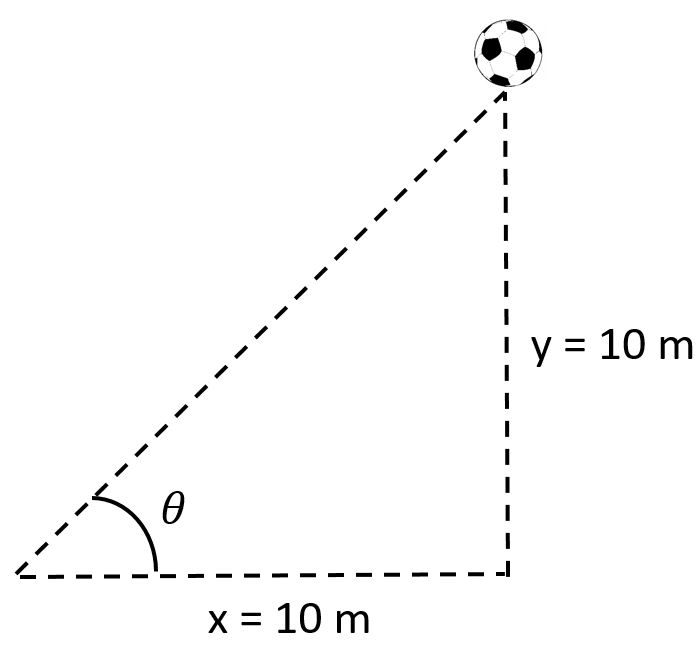
\includegraphics[width=\textwidth]{figures/LLp12ball}
	\end{minipage}\hfill
	\begin{minipage}{0.6\textwidth}
		\begin{itemize}
			\item \textbf{Aim:} calculate angle $\theta$
			\item[]
			\item using trigonometry, $\tan(\theta) = y/x$
			\item[]
			\item \textbf{Algorithm:} $\theta = \tan^{-1}(y/x)$
			\item[]
			\item Math review: $\tan^{-1}(z)$ calculates the angle $\theta$ such that $\tan(\theta)=z$
		\end{itemize}
	\end{minipage}
\end{figure}

\end{frame}

%==============================================================

\begin{frame}[fragile]
\frametitle{The program}

\begin{figure}[ht]
	\centering
	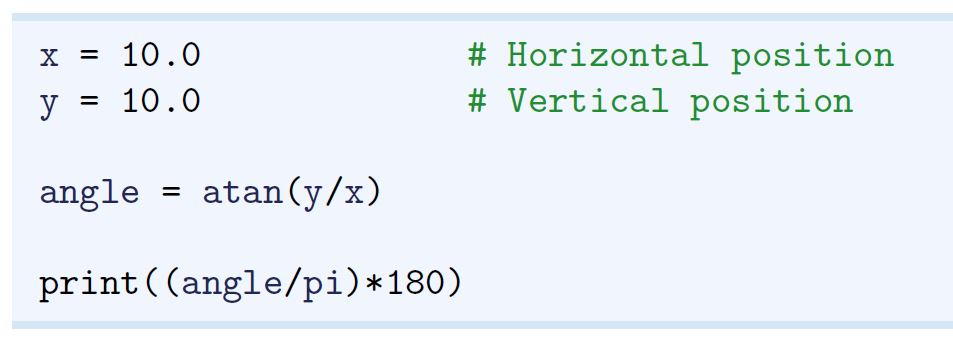
\includegraphics[width=\textwidth]{figures/LLp12}
\end{figure}

\begin{center}
\texttt{ball\_angle\_first\_try.py}
\end{center}

\end{frame}

%==============================================================

\begin{frame}[fragile]
\frametitle{First use of a Python function}

\begin{figure}[ht]
	\centering
	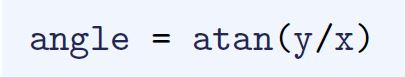
\includegraphics[width=0.5\textwidth]{figures/LLp12a}
\end{figure}

\begin{itemize}
	\item our first use of a \red{\emph{function}}, in this case \texttt{atan}
	\begin{itemize}
		\item corresponds to $\tan^{-1}$ in mathematics
	\end{itemize}
	\item line of code above shows how function \texttt{atan} is \red{\emph{called}}
	\item ratio $y/x$ is the \red{\emph{argument}} of function \texttt{atan}
	\item computed value is \red{\emph{returned}} from \texttt{atan}
	\begin{itemize}
		\item \ldots and result is assigned to \texttt{angle}
	\end{itemize}
\end{itemize}

\end{frame}

%==============================================================

\begin{frame}[fragile]
\frametitle{Math review: radians and degrees}

\begin{figure}[ht]
	\centering
	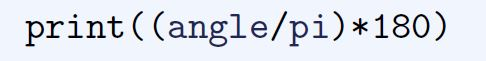
\includegraphics[width=0.5\textwidth]{figures/LLp12b}
\end{figure}

\begin{itemize}
\item Python's \texttt{atan} function returns angle in \emph{radians}
\item[]
\item multiply radians by $180/\pi$ to convert to degrees
\item[]
\end{itemize}
\end{frame}

%==============================================================

\begin{frame}[fragile]

\frametitle{Running the program in PyCharm}

\begin{figure}[ht]
	\centering
	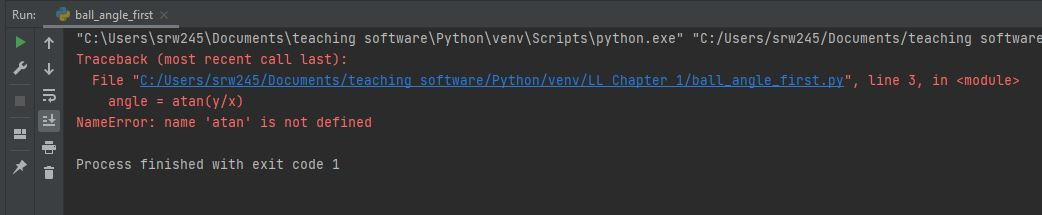
\includegraphics[width=\textwidth]{figures/LLp12output}
\end{figure}

\begin{verbatim}
 angle = atan(y/x) \\
NameError: name 'atan' is not defined
\end{verbatim}

\begin{itemize}
\item \textbf{Problem:} Python does not have \texttt{atan} \\ \qquad\qquad\quad function ``built-in''!
\end{itemize}

\end{frame}

%==============================================================

\begin{frame}[fragile]
\frametitle{Python standard library and import}

\begin{itemize}
	\item Python has some functionality built-in
	\item \ldots but LOTS more can be \red{\emph{imported}}
	\item \texttt{atan} and other trigonometric functions not built in
	\item to activate that functionality, must explicitly import
	\item \texttt{atan} function is grouped together with many other mathematical functions in a \red{\emph{library module}}  called \texttt{math}
\end{itemize}

\begin{figure}[ht]
	\centering
	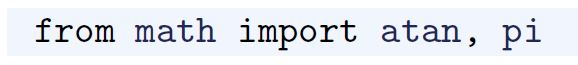
\includegraphics[width=0.6\textwidth]{figures/LLp13a}
\end{figure}

\end{frame}

%==============================================================

\begin{frame}[fragile]

\frametitle{The program: second attempt}

\begin{figure}[ht]
	\centering
	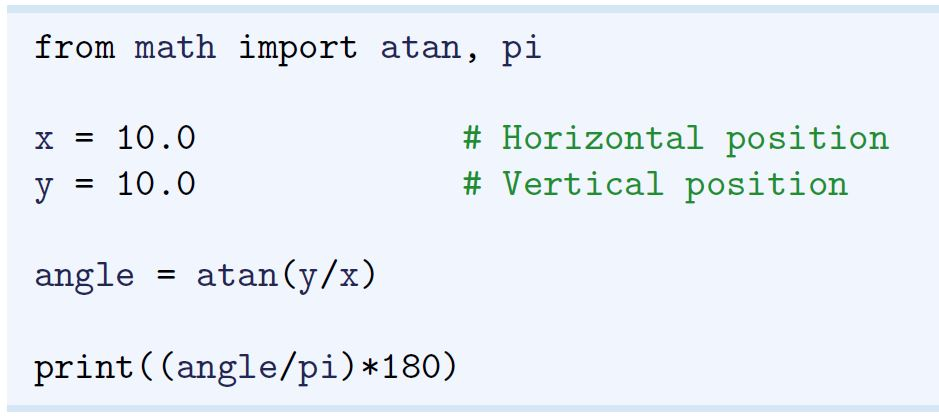
\includegraphics[width=0.9\textwidth]{figures/LLp13b}
\end{figure}
\begin{center}
	\texttt{ball\_angle.py}
\end{center}
\begin{itemize}
	\item script correctly produces $45.0$ as output
	\item live demo in PyCharm shortly
\end{itemize}

\end{frame}

%==============================================================

\begin{frame}[fragile]
\frametitle{Another way of importing}

\begin{itemize}
	\item use the import statement import math, but require \texttt{atan} and \texttt{pi} to be \red{\emph{prefixed}} with math
	\item both techniques are commonly used and are the two basic ways of importing library code in Python
\end{itemize}
\begin{figure}[ht]
	\centering
	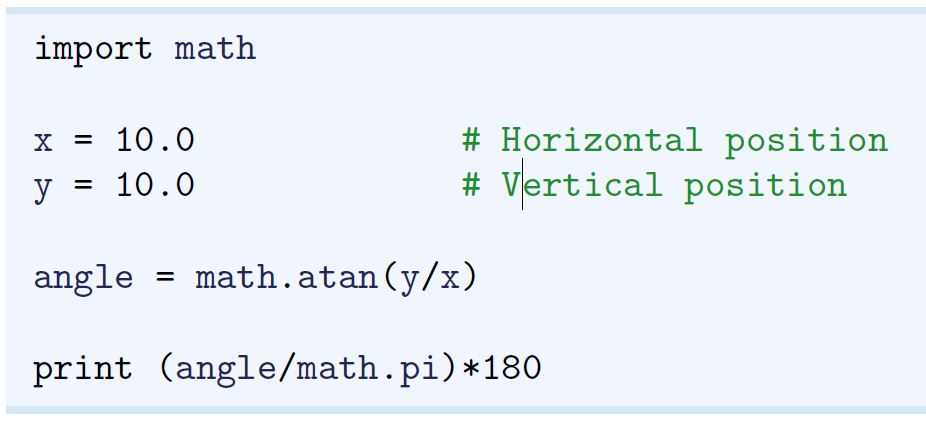
\includegraphics[width=0.7\textwidth]{figures/LLp14}
\end{figure}
\vspace*{-5mm}
\begin{center}
	\texttt{ball\_angle\_prefix.py}
\end{center}

\end{frame}

%==============================================================

\begin{frame}[fragile]
\frametitle{Live demo of Python program with a library function}

\end{frame}

%==============================================================

\begin{frame}[fragile]

\frametitle{$2)$ Importing from modules and packages}

\begin{itemize}
	\item Python has many libraries
	\item importing what's needed (and only what's needed) is sensible
\end{itemize}

\begin{itemize}
	\item[(a)] importing for use \textbf{\emph{without}} prefix %, eg: \texttt{ball\_angle.py}

	\item[]

	\item[(b)] importing for use \textbf{\emph{with}} prefix %, eg: \texttt{ball\_angle\_prefix.py}
	
	\begin{itemize}
		\item standard (and preferred) way to import
	\end{itemize}

\end{itemize}

\end{frame}

%==============================================================

\begin{frame}[fragile]
\frametitle{Importing for use \emph{without} prefix}

\begin{figure}[ht]
	\centering
	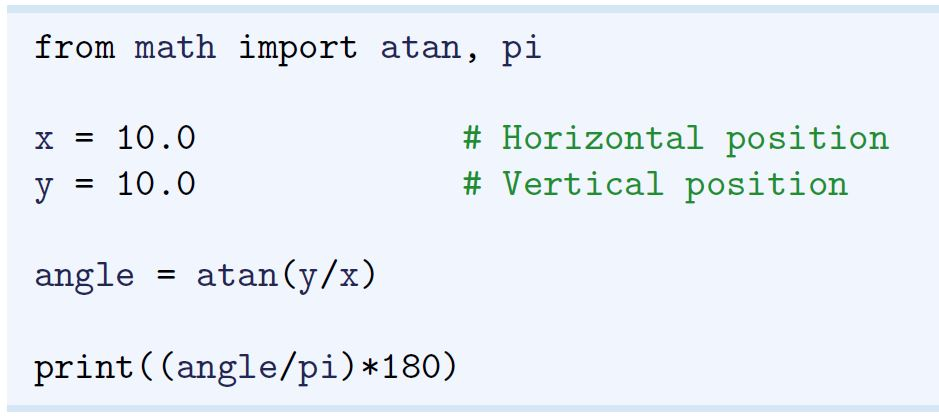
\includegraphics[width=0.8\textwidth]{figures/LLp13b}
\end{figure}
\begin{itemize}
	\item[\green{\cmark}] Python code is easier to read
	\item[\red{\xmark}] allows name conflicts!
\end{itemize}

\end{frame}

%==============================================================

\begin{frame}[fragile]

\frametitle{Name conflicts}

\begin{itemize}
	\item two libraries may each contain function with same name
\end{itemize}

\begin{figure}[ht]
	\centering
	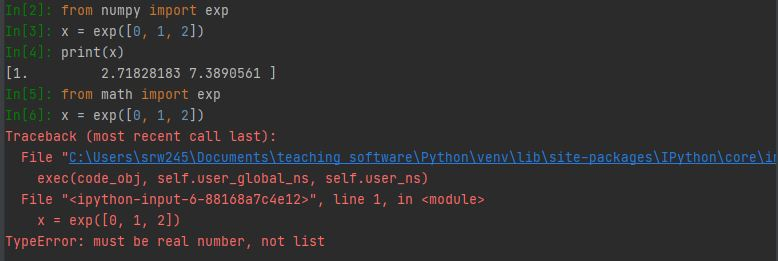
\includegraphics[width=0.9\textwidth]{figures/LLp16}
\end{figure}

{\small
\begin{itemize}
	\item[\green{\cmark}] \texttt{x = exp([0, 1, 2])} using \texttt{exp} from \textbf{numpy} works
	\item[\red{\xmark}] \texttt{x = exp([0, 1, 2])} using \texttt{exp} from \textbf{math} does not!
\end{itemize}
}
\end{frame}

%==============================================================

\begin{frame}[fragile]

\frametitle{Importing for use \emph{with} prefix}

\begin{figure}[ht]
	\centering
	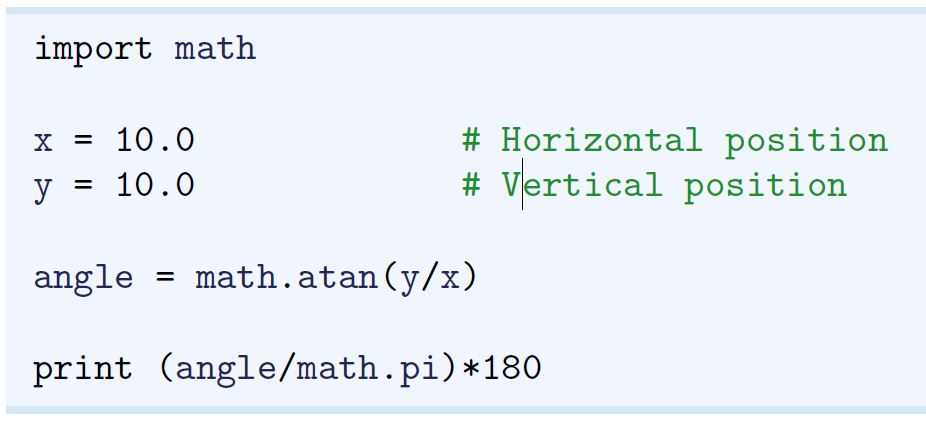
\includegraphics[width=0.8\textwidth]{figures/LLp14}
\end{figure}
\begin{itemize}
	\item[\red{\xmark}] Python code is a little harder for humans to read
	\item[\green{\cmark}\green{\cmark}] eliminates name conflicts!
	\item \textbf{import with prefix is the standard and safer and preferred method of importing}
\end{itemize}

\end{frame}

%==============================================================

\begin{frame}[fragile]

\frametitle{Avoiding name conflict using prefixes}

\begin{figure}[ht]
	\centering
	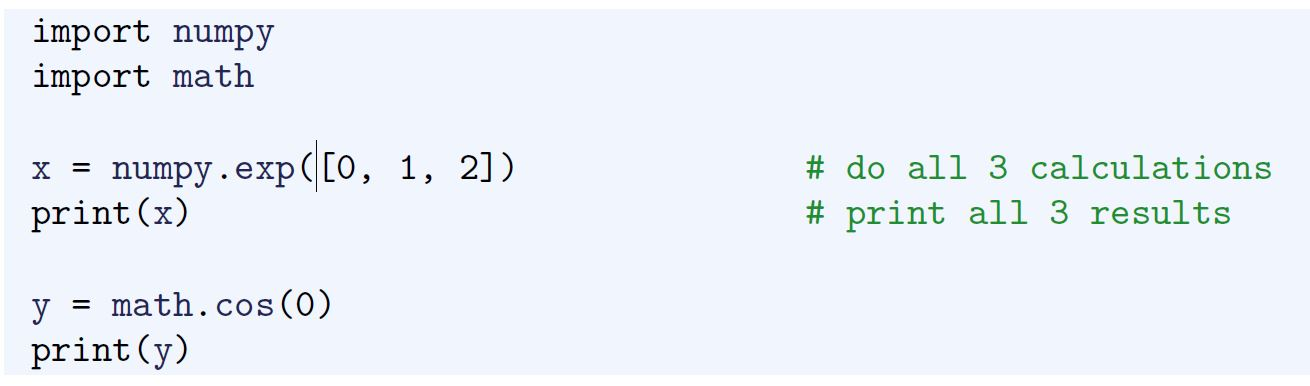
\includegraphics[width=0.8\textwidth]{figures/LLp17}
\end{figure}
\begin{itemize}
	\item \texttt{numpy} library includes an \texttt{exp} function
	\begin{itemize}
		\item math review:~exponential function $e^{z} =$~\texttt{exp(z)}
	\end{itemize}
	\item \texttt{math} library also includes an \texttt{exp} function---with a different implementation!
	\item[\green{\cmark}] \textbf{prefixes make clear which \texttt{exp} to use}
\end{itemize}

\end{frame}

%==============================================================

\begin{frame}[fragile]

\frametitle{Imports with name change}

\begin{figure}[ht]
	\centering
	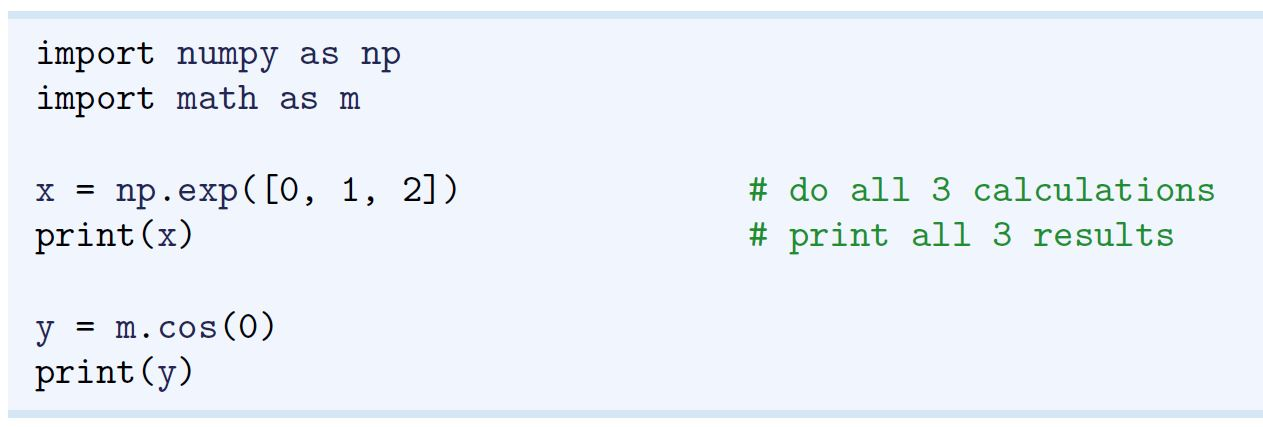
\includegraphics[width=0.9\textwidth]{figures/LLp18}
\end{figure}
\vspace*{-8mm}
\begin{itemize}
	\item using \red{as}, \texttt{numpy} name becomes \texttt{np} (``nickname'')
	\item similar for \texttt{math} and \texttt{m}
	\item[\green{\cmark}] Python code is easy to read
	\item[\green{\cmark}\green{\cmark}] eliminates name conflicts
\end{itemize}

\end{frame}

%==============================================================

\begin{frame}[fragile]

\frametitle{Main libraries used in ENGG1003}
\begin{itemize}
	\item \red{\textbf{\texttt{math}}}---basic mathematical operations \& constants
	\begin{itemize}
		\item math functions defined in C programming language
	\end{itemize}
	\item[]
	\item \red{\textbf{\texttt{numpy}}}---numerical Python
	\begin{itemize}
		\item large collection of powerful mathematical functions for scientific computing
		\item handles large datasets, matrices and arrays
	\end{itemize}
	\item[]
	\item \red{\textbf{\texttt{matplotlib}}}---visualization
	\begin{itemize}
		\item comprehensive library for creating static, animated, and interactive visualizations
		\item syntax closely follows MATLAB programming language
	\end{itemize}


\end{itemize}

\end{frame}

%==============================================================

\begin{frame}[fragile]

\frametitle{Live demo of importing}

\end{frame}

%==============================================================

\begin{frame}[fragile]

\frametitle{3) Simple plotting}

\begin{itemize}
	\item from week 1 lecture, vertical position $y$ of ball at time $t$:
	\[
		y = v_0 t - 0.5gt^2
	\]
	\begin{itemize}
		\item $v_0$ is initial upwards velocity ($\mathrm{m/s}$)
		\item $g = 9.81$ is acceleration due to gravity ($\mathrm{m/s^2}$)
		\item given $v_0$ and $t$, can calculate $y$
	\end{itemize}
	
	\item now want to calculate height $y$ at every millisecond for first second of flight
	\item \ldots and plot $y$ graphically with time $t$
\end{itemize}


\end{frame}

%==============================================================

\begin{frame}[fragile]

\frametitle{Simple plot program}

\vspace*{-6mm}
\begin{center}
{\small
\texttt{ball\_plot.py}
}
\end{center}
\vspace*{-8mm}
\begin{figure}[ht]
	\centering
	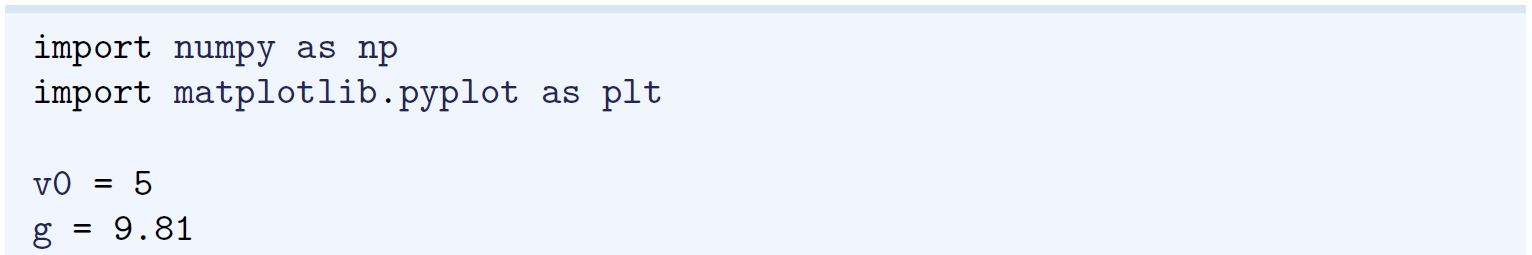
\includegraphics[width=0.9\textwidth]{figures/LLp19}
	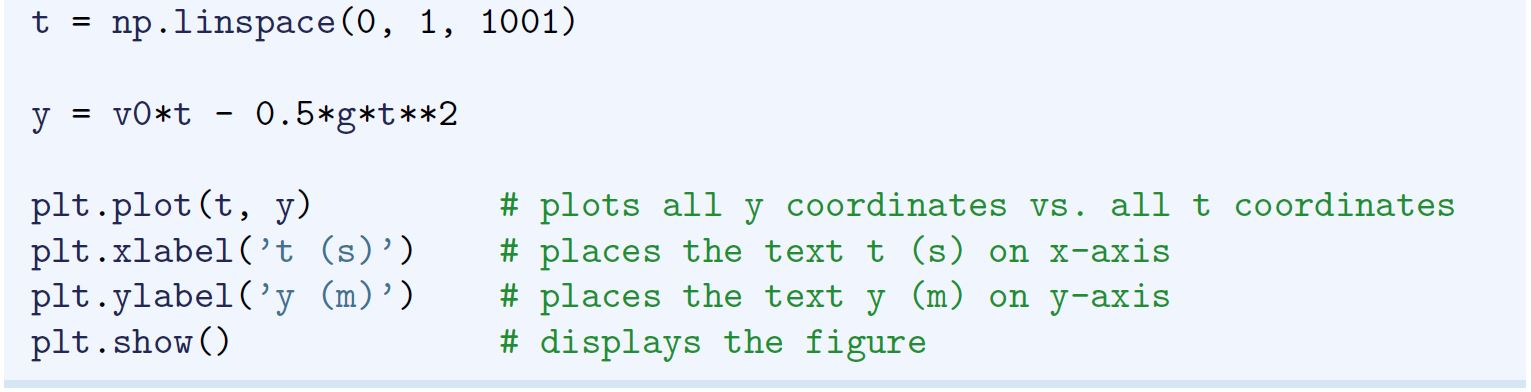
\includegraphics[width=0.9\textwidth]{figures/LLp20a}
\end{figure}
\vspace*{-8mm}
\begin{itemize}
	\item \texttt{linspace} function and our first \red{\emph{array}}
	\item \red{\emph{vectorization}} in \texttt{y = v0*t - 0.5*g*t**2}
	\item plot commands
\end{itemize}

\end{frame}

%==============================================================

\begin{frame}[fragile]

\frametitle{Program output}

When we run \texttt{ball\_plot.py} in PyCharm:
\begin{figure}[ht]
	\centering
	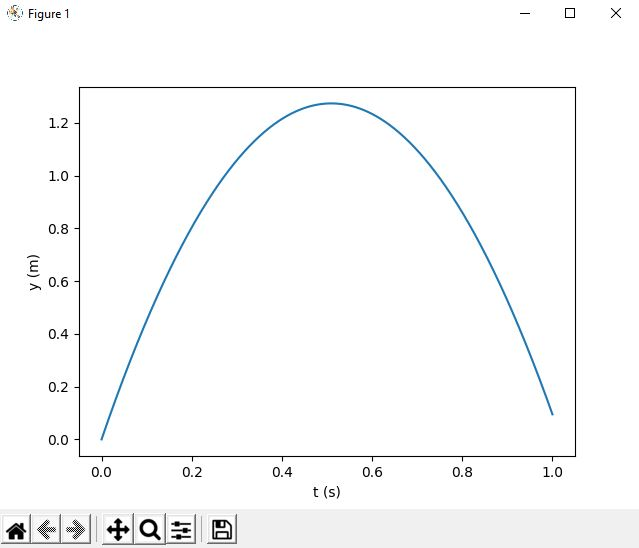
\includegraphics[width=0.6\textwidth]{figures/LLp20output}
\end{figure}

\end{frame}

%==============================================================

\begin{frame}[fragile]

\frametitle{Our first array}

\begin{figure}[ht]
	\centering
	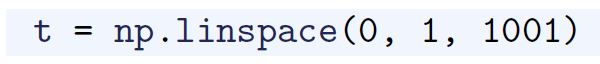
\includegraphics[width=0.7\textwidth]{figures/LLp20b}
\end{figure}
\vspace*{-8mm}
\begin{itemize}
	\item creates $1001$ coordinates on the interval $[0,1]$:
	\item[] $0, 0.001, 0.002, \ldots, 1$
	\item Python stores these as an \red{\emph{array}}
	\item think of the array \texttt{t} as a collection of ``boxes'' in computer memory
	\item Python numbers these boxes consecutively from zero upwards:
	\item[] \texttt{t[0], t[1], t[2], \ldots, t[1000]}
\end{itemize}

\end{frame}

%==============================================================

\begin{frame}[fragile]
\frametitle{Vectorization}

\vspace*{-4mm}
\begin{figure}[ht]
	\centering
	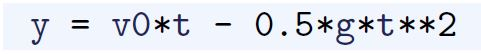
\includegraphics[width=0.6\textwidth]{figures/LLp21a}
\end{figure}
\vspace*{-4mm}

\begin{itemize}
	\item right-hand side is computed for every entry in the array \texttt{t}
	\item ie: for \texttt{t[0], t[1], t[2], \ldots, t[1000]}
	\item[\green{\cmark}] yields a collection of 1001 numbers in the result \texttt{y}, which
	(automatically) also becomes an array!
	\item technique of computing all numbers ``in one chunk'' is called \red{\emph{vectorization}}
\end{itemize}

\end{frame}

%==============================================================

\begin{frame}[fragile]

\frametitle{Plotting commands}

Plotting commands are new, but simple:

\begin{figure}[ht]
	\centering
	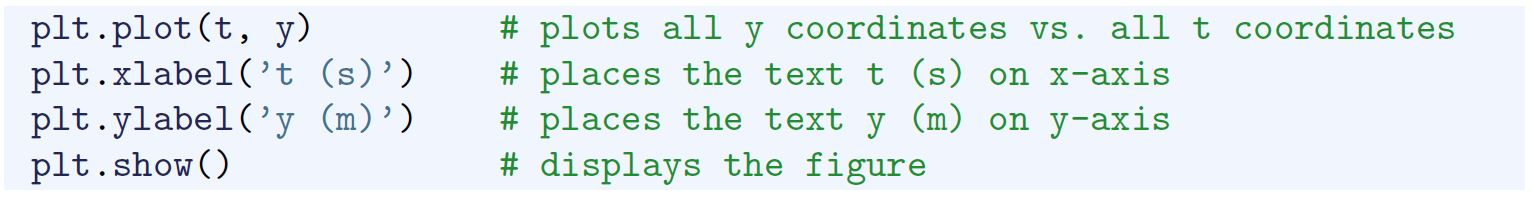
\includegraphics[width=\textwidth]{figures/LLp21b}
\end{figure}

\end{frame}

%==============================================================

\begin{frame}[fragile]

\frametitle{Live demo of simple plotting}

\end{frame}

%==============================================================

\begin{frame}[fragile]
\frametitle{4) Plotting and printing}

\begin{itemize}
	\item \texttt{Matplotlib} is standard plotting package in Python
	\item have already seen array \texttt{y} (heights) plotted against another array \texttt{t} (points in time) 
\end{itemize}
\vspace*{-6mm}
\begin{center}
{\small\blue{
\textbf{
\texttt{plt.plot(t,y)}}}
}
\end{center}
\vspace*{-8mm}
\begin{figure}[ht]
	\centering
	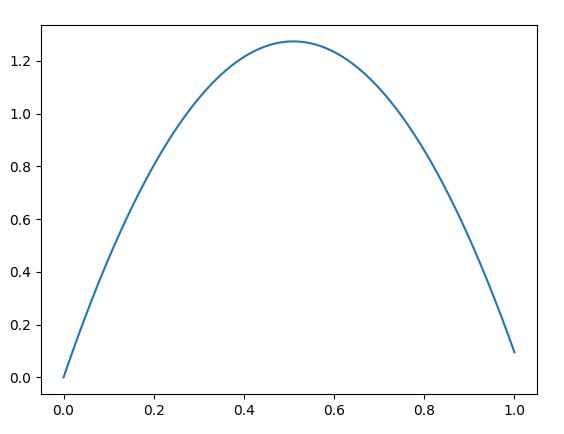
\includegraphics[width=0.4\textwidth]{figures/LLp22a}
\end{figure}

\end{frame}

%==============================================================

\begin{frame}[fragile]
\frametitle{Line styles}

\begin{figure}[ht]
	\centering
	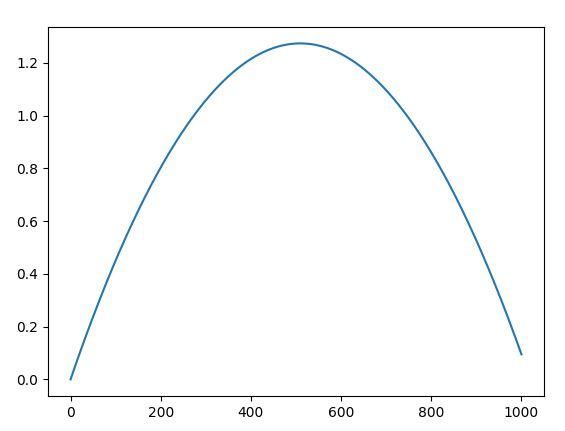
\includegraphics[width=0.5\textwidth]{figures/LLp23aoutput}%
	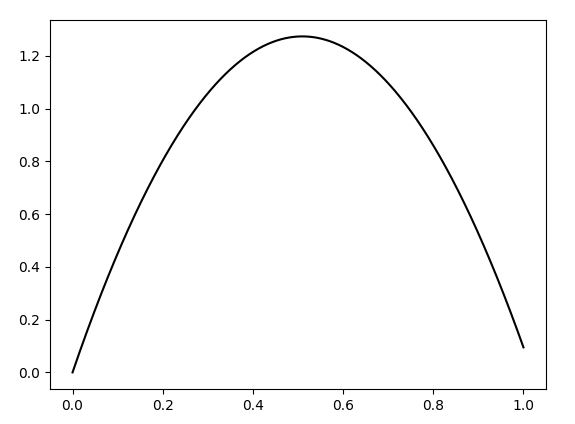
\includegraphics[width=0.5\textwidth]{figures/LLp23boutput}
\end{figure}
\vspace*{-8mm}
\begin{itemize}
	\item[left:] \texttt{plt.plot(y) \# x-axis indices}
	\item[right:] \texttt{plt.plot(t, y, 'k')  \# black line}
\end{itemize}

\end{frame}

%==============================================================

\begin{frame}[fragile]
\frametitle{More line styles}

\begin{figure}[ht]
	\centering
	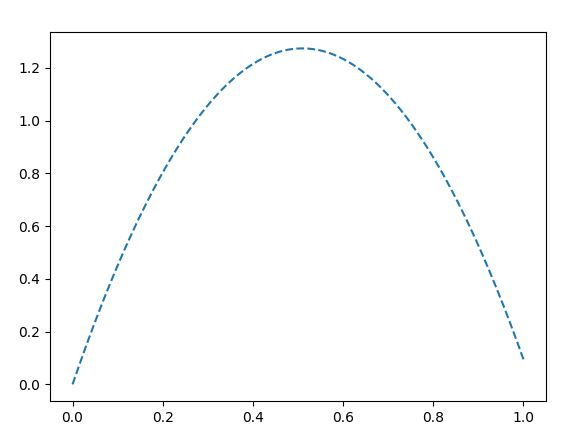
\includegraphics[width=0.5\textwidth]{figures/LLp23coutput}%
	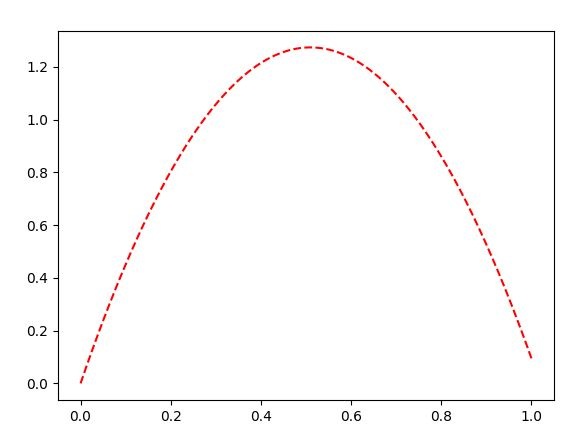
\includegraphics[width=0.5\textwidth]{figures/LLp23doutput}
\end{figure}
\vspace*{-8mm}
\begin{itemize}
	\item[left:] \texttt{plt.plot(t, y, '--') \# dashed}
	\item[right:] \texttt{plt.plot(t, y, 'r--') \# red dashed}
\end{itemize}

\end{frame}

%==============================================================

\begin{frame}[fragile]
\frametitle{Plotting points only}

\begin{figure}[ht]
	\centering
	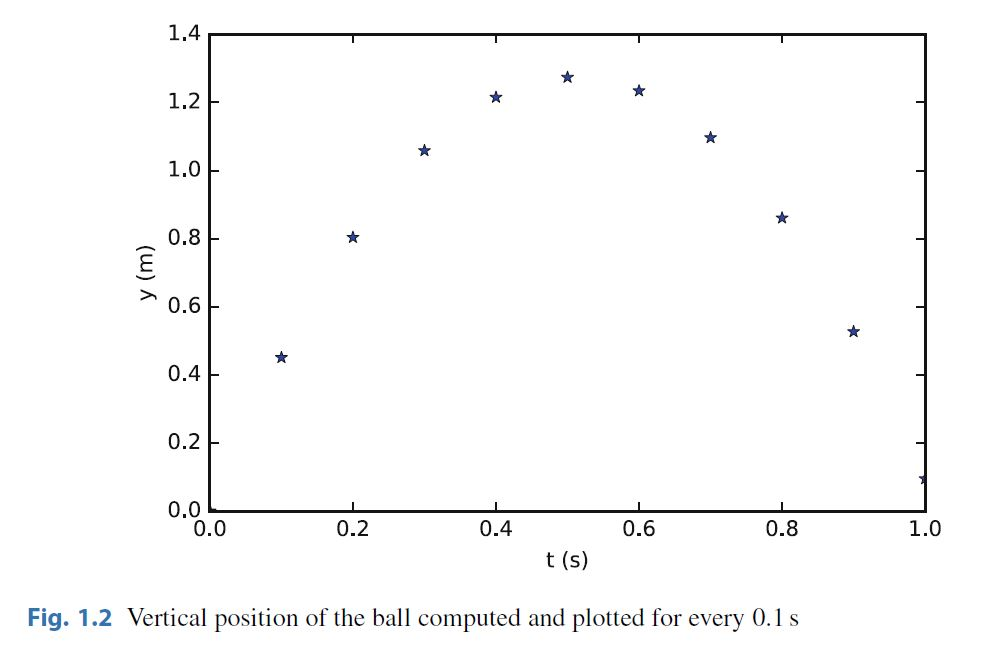
\includegraphics[width=0.7\textwidth]{figures/LLp24a}
	
\includegraphics[width=\textwidth]{figures/LLp23a}
	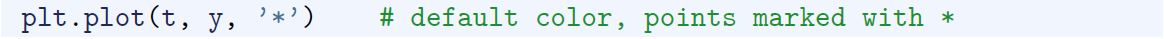
\includegraphics[width=\textwidth]{figures/LLp23b}
\end{figure}

\end{frame}

%==============================================================

\begin{frame}[fragile]
\frametitle{Decorating a plot}

\vspace*{-3mm}
\begin{figure}[ht]
	\centering
	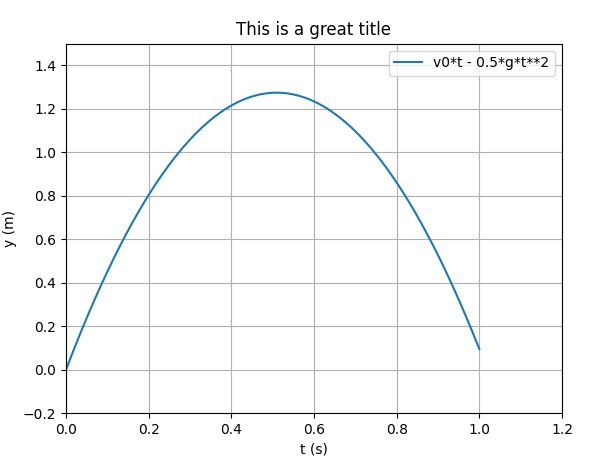
\includegraphics[width=0.8\textwidth]{figures/LLp24output}
\end{figure}

\end{frame}

%==============================================================

\begin{frame}[fragile]
\frametitle{Decorating a plot}

\begin{itemize}
	\item add a legend
	\vspace*{-5mm}
	\begin{figure}[ht]
		\centering
		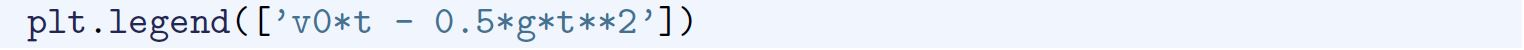
\includegraphics[width=\textwidth]{figures/LLp24c}
	\end{figure}

	\item add a grid
	\vspace*{-5mm}
	\begin{figure}[ht]
		\centering
		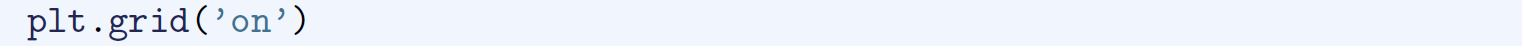
\includegraphics[width=\textwidth]{figures/LLp24d}
	\end{figure}
	\item display a title
\vspace*{-5mm}
	\begin{figure}[ht]
		\centering
		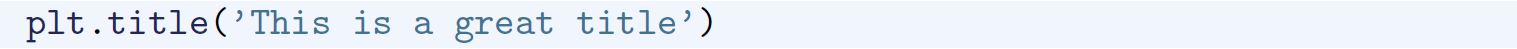
\includegraphics[width=\textwidth]{figures/LLp24e}
	\end{figure}
	\item override default ranges for plot axes
	\vspace*{-5mm}
	\begin{figure}[ht]
		\centering
		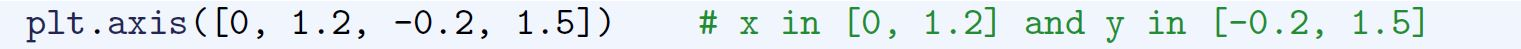
\includegraphics[width=\textwidth]{figures/LLp24f}
	\end{figure}
\end{itemize}

\end{frame}

%==============================================================

\begin{frame}[fragile]
\frametitle{Multiple curves in the same plot}

\begin{figure}[ht]
	\centering
	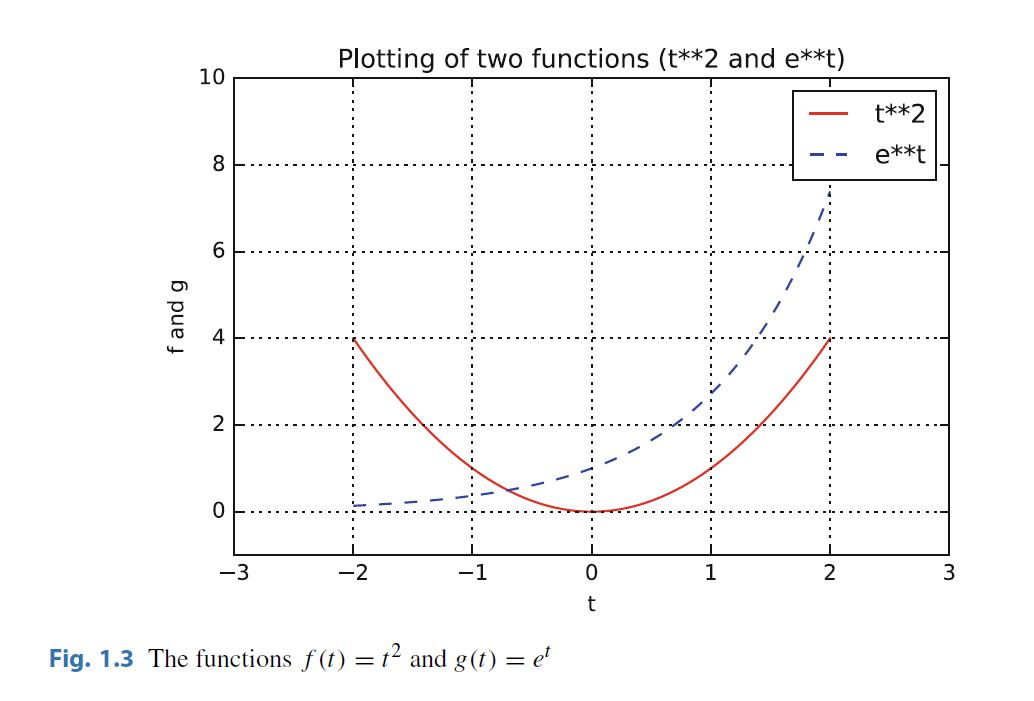
\includegraphics[width=0.9\textwidth]{figures/LLp25b}
\end{figure}

\end{frame}

%==============================================================

\begin{frame}[fragile]
\frametitle{Multiple curves in the same plot}

\vspace*{-3mm}
\begin{figure}[ht]
	\centering
	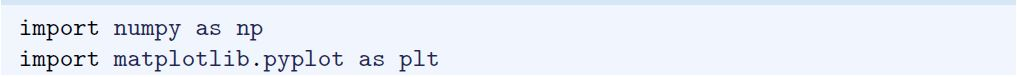
\includegraphics[width=0.9\textwidth]{figures/LLp24b}
	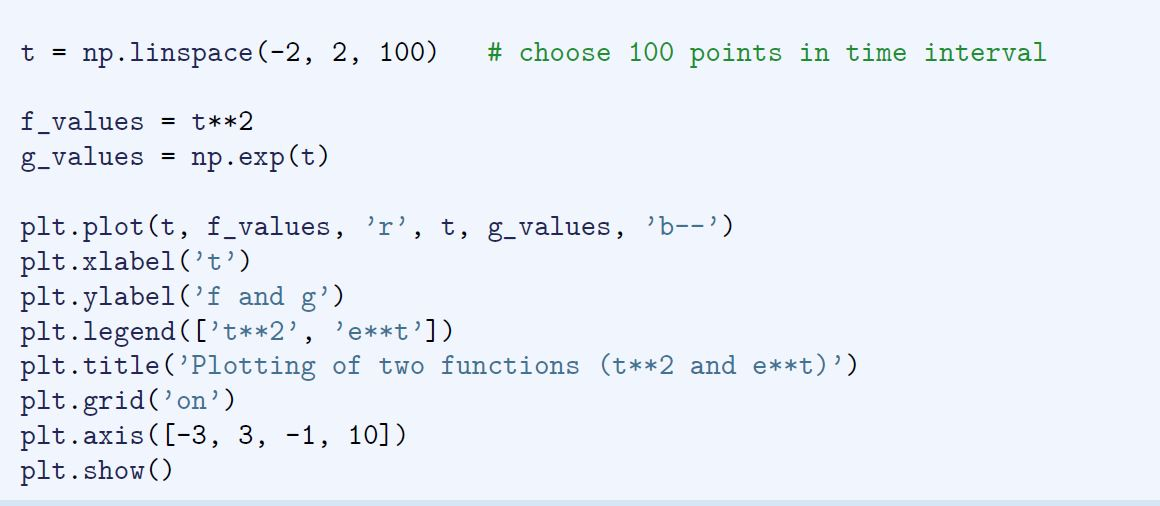
\includegraphics[width=0.9\textwidth]{figures/LLp25a}
\end{figure}
\vspace*{-3mm}
Key line of code for multiple curves:
\begin{figure}[ht]
	\centering
	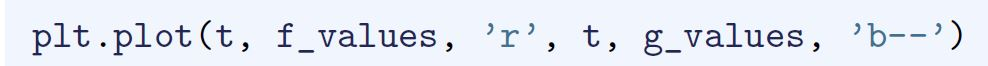
\includegraphics[width=0.7\textwidth]{figures/LLp25c}
\end{figure}

\end{frame}

%==============================================================

\begin{frame}[fragile]
\frametitle{Printing variables and strings}

\begin{itemize}
\item print the value of variable \texttt{y}

\begin{figure}[ht]
	\centering
	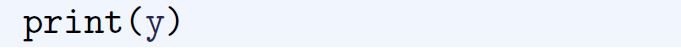
\includegraphics[width=0.8\textwidth]{figures/LLp27a}
\end{figure}

\vspace*{10mm}
\item print the string \texttt{This is some text}
\begin{figure}[ht]
	\centering
	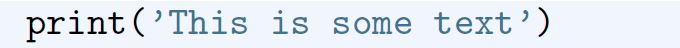
\includegraphics[width=0.8\textwidth]{figures/LLp27b}
\end{figure}
	\begin{itemize}
		\item enclose text in single quotes
	\end{itemize}
\end{itemize}

\end{frame}

%==============================================================

\begin{frame}[fragile]

\frametitle{Print \emph{one} variable and text combined}

\begin{itemize}
\item if variable \texttt{v1} has value $10.0$ and you want to display as follows:

\begin{figure}[ht]
	\centering
	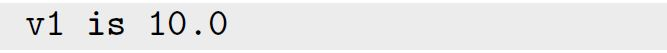
\includegraphics[width=0.8\textwidth]{figures/LLp28a}
\end{figure}

\item use the following Python code:
\begin{figure}[ht]
	\centering
	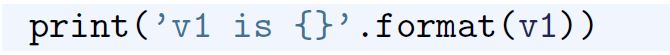
\includegraphics[width=0.8\textwidth]{figures/LLp28b}
\end{figure}
	\begin{itemize}
		\item pair of curly brackets \{\} acts as a \red{\emph{placeholder}}
		\item \ldots says \emph{where} to place value
		\item \texttt{.format(v1)} converts variable \texttt{v1} to string \texttt{10.0}
	\end{itemize}
\end{itemize}

\end{frame}

%==============================================================

\begin{frame}[fragile]
\frametitle{Printing \emph{several} variables and text combined}

\begin{itemize}
\item if \texttt{v1} and \texttt{v2} have values $10.0$ and $20.0$ and you want to display as follows:

\begin{figure}[ht]
	\centering
	
\includegraphics[width=0.8\textwidth]{figures/LLp28d}
\end{figure}

\item use the following Python code:
\begin{figure}[ht]
	\centering
	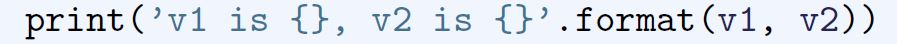
\includegraphics[width=0.8\textwidth]{figures/LLp28c}
\end{figure}
\vspace*{-3mm}
	\begin{itemize}
		\item now \emph{two} pairs of curly brackets \{\} act as a placeholders
		\item \texttt{.format(v1,v2)} dictates the order in which placeholders are filled
		\item in this case: \texttt{v1} first, then \texttt{v2}
	\end{itemize}
\end{itemize}

\end{frame}

%==============================================================

\begin{frame}[fragile]

\frametitle{Controlled printing: decimals, scientific notation \& strings}

\begin{itemize}
\item[] 	\begin{itemize}
		\item real number $12.89643$
		\item integer $42$
		\item string \texttt{some message}
	\end{itemize}

\item suppose you want to display as follows:
\begin{figure}[ht]
	\centering
	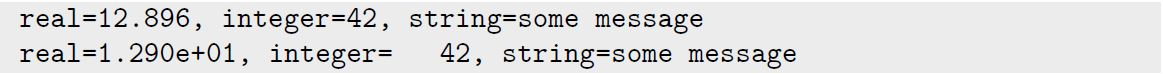
\includegraphics[width=0.8\textwidth]{figures/LLp29a}
\end{figure}

\item use the following Python code:
\begin{figure}[ht]
	\centering
	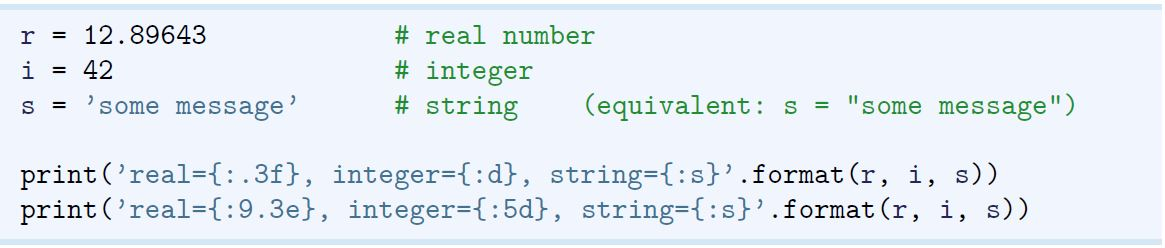
\includegraphics[width=0.8\textwidth]{figures/LLp29b}
\end{figure}

\end{itemize}

\end{frame}

%==============================================================

\begin{frame}[fragile]

\frametitle{Controlled printing: decimals, scientific notation \& strings}

\begin{itemize}
\item first call to \texttt{print}

\begin{figure}[ht]
	\centering
	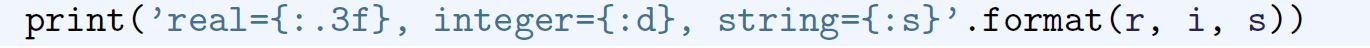
\includegraphics[width=0.9\textwidth]{figures/LLp30a}
\end{figure}
\vspace*{-3mm}
	\begin{itemize}
		\item \texttt{:.3f} \quad write number \texttt{r} compactly using 3 decimals
		\item \texttt{:d} \quad~~~ write integer \texttt{i} as compactly as possible
		\item \texttt{:s} \quad\quad~\!\! write string \texttt{s}
	\end{itemize}
	
\item second call to \texttt{print}
\begin{figure}[ht]
	\centering
	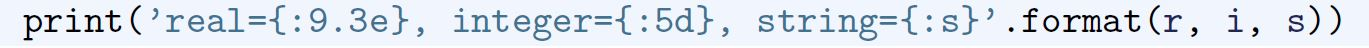
\includegraphics[width=0.9\textwidth]{figures/LLp30b}
\end{figure}
\vspace*{-3mm}
	\begin{itemize}
		\item \texttt{:9.3e} \quad write number \texttt{r} in \red{\emph{scientific notation}} with \\
		\qquad\qquad\qquad $3$ decimals in field of width $9$ characters
		\item \texttt{:5d} \quad~~~ write integer \texttt{i} in field of width $5$ characters
	\end{itemize}
\end{itemize}

\end{frame}

%==============================================================

\begin{frame}[fragile]
\frametitle{Live demo of plotting and printing}

\end{frame}

\end{document}
